\newpage
\section{File-System Interface}

\begin{figure}[!htb]
    \centering
    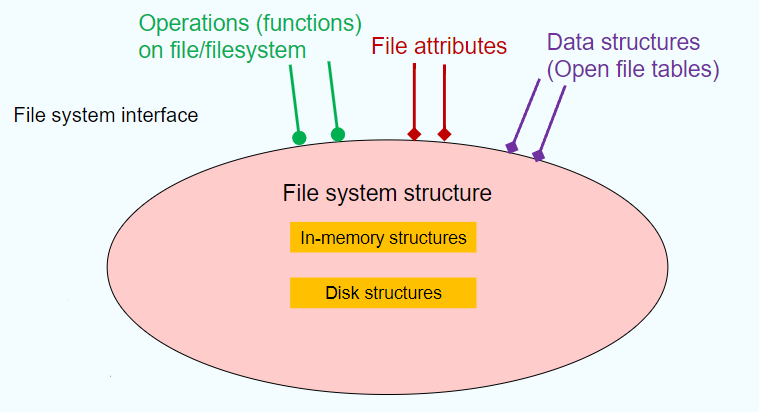
\includegraphics[width=0.309\textwidth]{pic/OS10/Mind Map for Ch10 and 11}
    \caption{Mind Map for Ch10 and 11}
\end{figure}

\subsection{File Concept}
\begin{definition}[File System]
    The way that controls how data is stored and retrieved in a storage medium
    \begin{itemize}
        \item File naming
        \item Where files are placed
        \item Metadata
        \item Access rules
    \end{itemize}
\end{definition}

\begin{definition}[File]
    Contiguous logical address space. 
    
    A sequence of bits, bytes, lines, or records. The meaning is defined by the creator and user.
\end{definition}

File Structure:
\begin{itemize}\scriptsize
    \item None: sequence of words, bytes
    \item Simple record structure: Lines, Fixed length, Variable length
    \item Complex Structures: Formatted document, Relocatable load file
\end{itemize}

\subsubsection{File Attributes}
\begin{itemize}\scriptsize
    \item Name: only information kept in human-readable form
    \item Identifier: unique tag (number) identifies file within file system
    \item Type: needed for systems that support different types
    \item Location: pointer to file location on device
    \item Size: current file size
    \item Protection: controls who can do reading, writing, executing
    \item Time, date, and user identification: data for protection, security,
    and usage monitoring
\end{itemize}
Information about files are kept in the directory structure, which is
maintained on the disk

\subsubsection{File Operations}
File is an abstract data type
\begin{itemize}\scriptsize
    \item Create
    \item Write: define a pointer
    \item Read: use the same pointer Per-process current file-position pointer
    \item Reposition within file (file seek)
    \item Delete
    \item Truncate(截取)
    \item Open($F_i$): search the directory structure on disk for entry $F_i$, and move the content of entry to memory
    \item Close ($F_i$): move the content of entry $F_i$ in memory to directory
    structure on disk
\end{itemize}

\subsubsection{Open-file table(打开文件表)}
Open() system call returns a pointer to an entry in the open-file table. 即打开文件就在 table 中写一个 entry. 

\begin{itemize}
    \item Per-process table, for $P_1$, $P_2$
    \item System-wide table, for OS kernel
\end{itemize}

若多个 process 打开一个文件, 需要使用 system-wide table 处理. 

\subsubsection{Open File Locking}
Provided by some operating systems and file systems. Mediates access to a file. Mandatory or advisory. 

\subsubsection{File Types}
\begin{figure}[!htb]
    \centering
    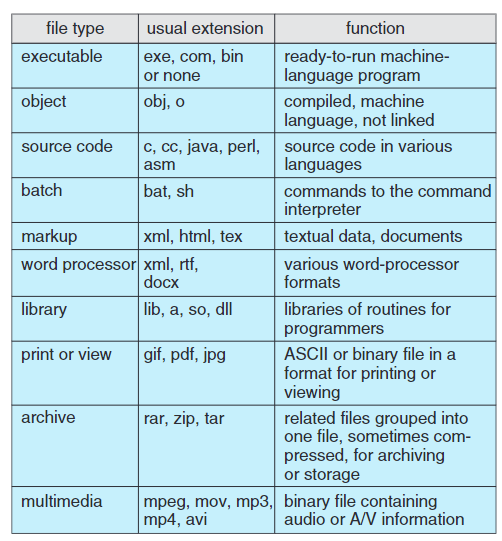
\includegraphics[width=0.309\textwidth]{pic/OS10/Common file types}
    \caption{Common file types}
\end{figure}

Linux 使用 Magic number 判断文件类型. 

\subsection{Access Methods}
\begin{itemize}
    \item Sequential Access
    \item Direct (Random) Access
\end{itemize}

\begin{figure}[!htb]
    \centering
    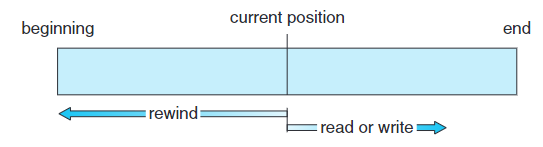
\includegraphics[width=0.309\textwidth]{pic/OS10/Sequential-access file}
    \caption{Sequential-access file}
\end{figure}

\begin{figure}[!htb]
    \centering
    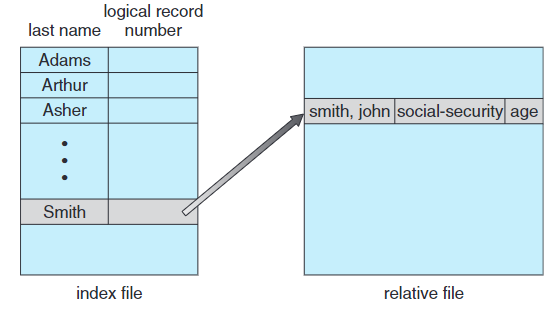
\includegraphics[width=0.309\textwidth]{pic/OS10/Example of index and relative files}
    \caption{Example of index and relative files}
\end{figure}


\subsection{Directory Structure}
A collection of nodes containing (management) information about all files. 

\begin{figure}[!htb]
    \centering
    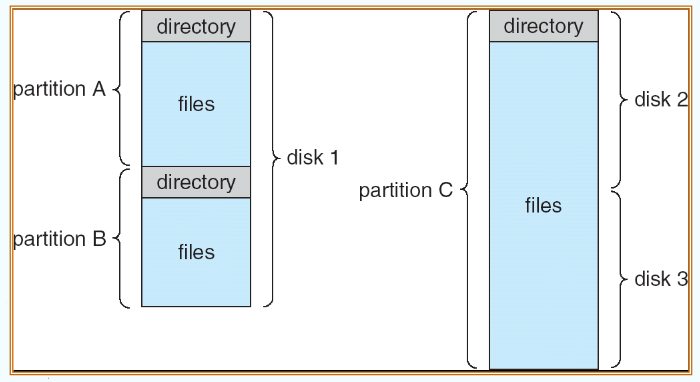
\includegraphics[width=0.309\textwidth]{pic/OS10/A Typical File-system Organization}
    \caption{A Typical File-system Organization}
\end{figure}

有 volume, 其中用 partition 存储 file. 

\subsubsection{Operations Performed on Directory}
\begin{itemize}\scriptsize
    \item Search for a file
    \item Create a file
    \item Delete a file
    \item List a directory
    \item Rename a file
    \item Traverse the file system – access every dir and file for backing up.
\end{itemize}

\subsubsection{Organize the Directory (Logically) to Obtain}
\begin{itemize}
    \item Efficiency: locating a file quickly
    \item Naming: convenient to users
    \item Grouping: logical grouping of files by properties
\end{itemize}

\subsubsection{Directory}%TODO 25-33
\begin{itemize}
    \item Single-Level Directory
    \item Two-Level Directory
    \item Tree-Structured Directories
    \item Acyclic-Graph Directories
    \item General Graph Directory
\end{itemize}

\subsubsection{Soft Link v.s. Hard Link}
%TODO 12.5 5:14 P34
\begin{itemize}
    \item Soft Link: a string
    \item Hard Link: a link
\end{itemize}


\subsection{File-System Mounting}
A file system must be mounted before it can be accessed. 

An un-mounted file system is mounted at a mount point. 

chroot: linux 中切换根目录. 

\subsection{Protection}
Types of access:
\begin{itemize}
    \item Read
    \item Write
    \item Execute
    \item Append
    \item Delete
    \item List
\end{itemize}


\subsubsection{Access Lists and Groups}
Mode of access: read, write, execute

\begin{figure}[!htb]%TODO to table
    \centering
    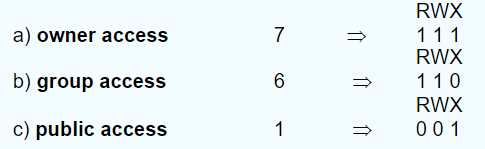
\includegraphics[width=0.309\textwidth]{pic/OS10/Three classes of users}
    \caption{Three classes of users}
\end{figure}


\begin{figure}[!htb]
    \centering
    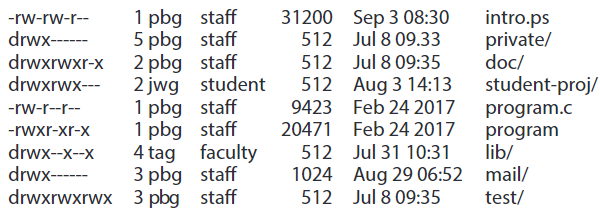
\includegraphics[width=0.309\textwidth]{pic/OS10/A Sample UNIX Directory Listing}
    \caption{A Sample UNIX Directory Listing}
\end{figure}
